\chapter{Conneciones UDP y TCP}

El servidor DNS implementado usa la librería \texttt{tokio} para atender consultas en UDP y TCP de forma asíncrona y concurrente. 
Además de la funcionalidad básica de recibir y devolver respuestas, también soporta EDNS0, detecta y respeta el payload máximo 
anunciado por el cliente en el registro OPT, maneja el estándar DNSSEC (lectura del bit DO) y protege operaciones críticas
con timeouts para evitar bloqueos y bucles infinitos. También se manejan correctamente errores de parseo (se responde FORMERR) y
se implementa el comportamiento para truncamiento (TC) sobre UDP con fallback a TCP.

A continuación se describen las implementaciones específicas para cada protocolo.

\section{UDP}

El servidor UDP está implementado en la estructura \texttt{ServerUDPConnection}, que contiene los siguientes campos y métodos:

\begin{table}[h!]
\centering
\renewcommand{\arraystretch}{1,1}

\begin{tabular}{|p{0.95\linewidth}|}
\hline
\multicolumn{1}{|c|}{\textbf{ServerUDPConnection}} \\
\hline
\textbf{Campos} \\
\hline
\texttt{- timeout: tokio::time::Duration} \\
\texttt{- payload\_size: usize} \\
\hline
\textbf{Métodos Públicos} \\
\hline
\texttt{+ new\_udp(timeout: Duration, payload\_size: usize) -> Self} \\
\texttt{+ new\_default(timeout: Duration) -> Self} \\
\texttt{+ receive\_and\_response(\&mut self) -> Result<(), ServerError>} \\
\hline
\textbf{Métodos Privados / Auxiliares} \\
\hline
\texttt{- handle\_dns\_message\_udp\_with\_timeout (} \\
\texttt{\ \ timeout\_server: Duration, recv\_buf: \&[u8],} \\
\texttt{\ \ socket: \&UdpSocket, client\_addr: SocketAddr,} \\
\texttt{\ \ tc\_case: bool, len: usize ) ->  Result<(), ServerError>} \\
\hline
\end{tabular}
\end{table}

%%Explicacion de los campos

El campo \texttt{timeout} define el tiempo máximo que el servidor esperará para recibir una consulta o enviar una respuesta antes de abortar la operación.
El campo \texttt{payload\_size} establece el tamaño máximo de la consulta DNS que el servidor puede procesar.

%%Explicacion de los metodos

Los métodos definidos incluyen funciones típicas como \texttt{new} y \texttt{new\_default}, que permiten crear 
una instancia de la clase con parámetros personalizados o por defecto. Sin embargo, la función más relevante es \texttt{receive\_and\_response}, 
la cual se encarga de recibir y responder de manera asíncrona a las consultas DNS enviadas por los clientes.

%%Explicación del flujo

La funcion \texttt{receive\_and\_response} sigue los siguientes pasos:
\begin{itemize}
    \item Crea un socket UDP y se enlaza a localhost en el puerto 53.
    \item Entra en un bucle infinito donde se espera recibir consultas DNS.
    \item Crean los distintos threads con \texttt{tokio} para manejar la concurrencia.
    \item En cada thread, si el tamaño de la consulta es mayor al \texttt{payload\_size}, se usa la función \texttt{handle\_dns\_message\_udp\_with\_timeout}
          con \texttt{tc\_case} en true, de lo contrario se llama a la misma función con \texttt{tc\_case} en false.
\end{itemize}

%Imagen del diagrama de flujo desde la carpeta diagramas, con 

\begin{figure}[h!]
    \centering
    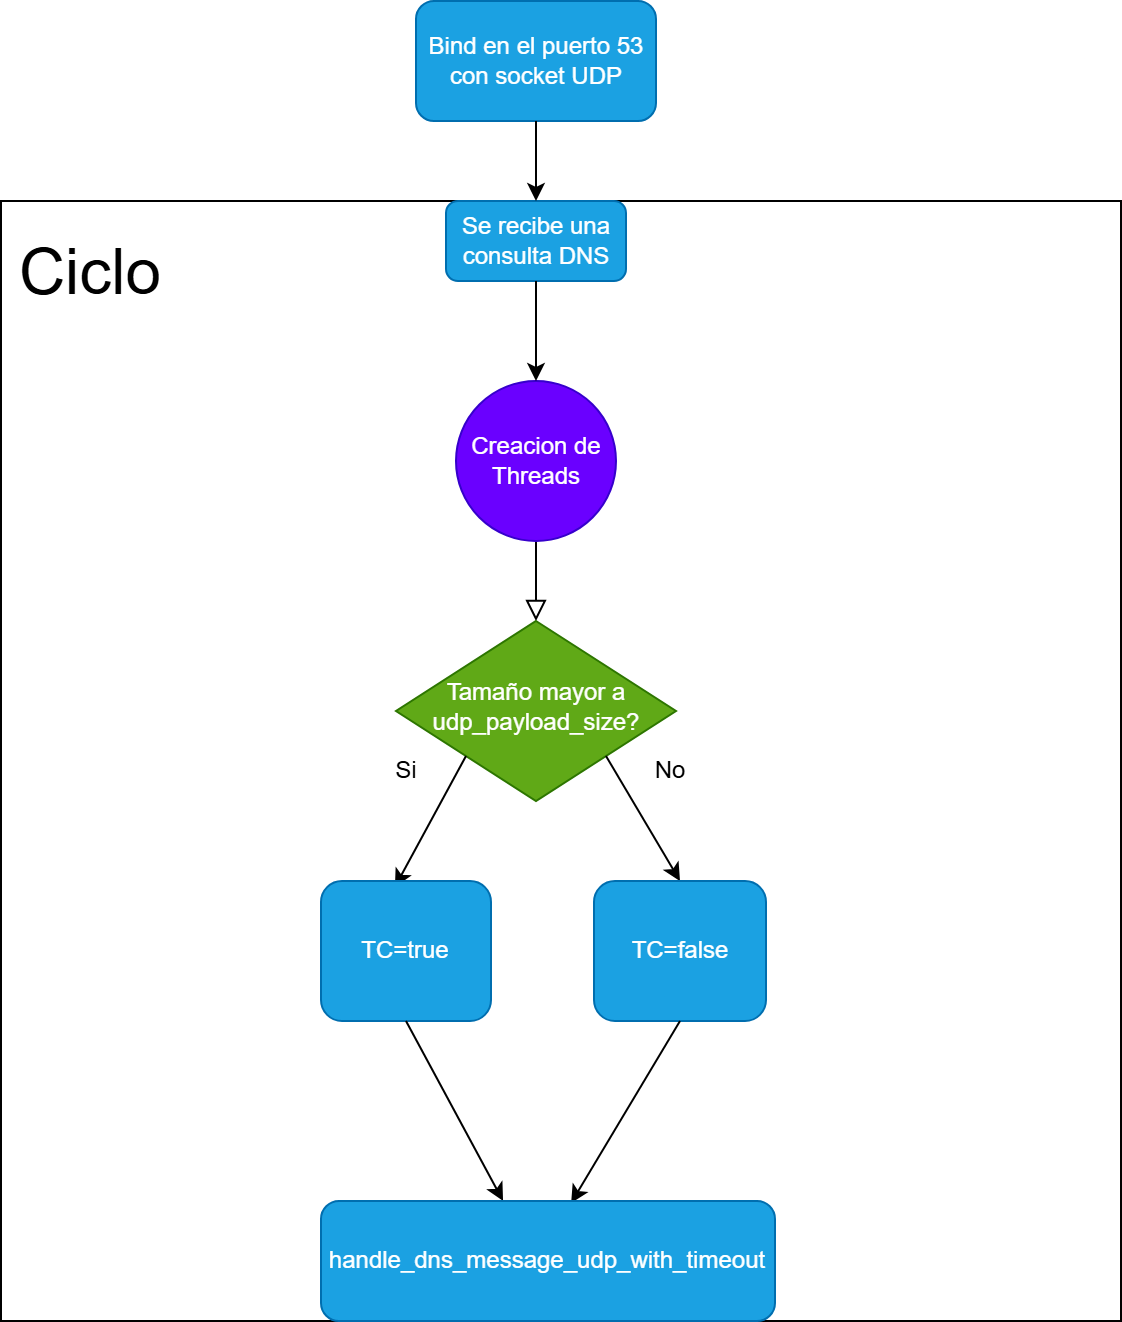
\includegraphics[width=0.7\textwidth]{diagramas/recieve_and_response.png}
    \label{fig:udp_flowchart}
\end{figure}


Con respecto a la función auxiliar \texttt{handle\_dns\_message\_udp\_with\_timeout}, esta se encarga de:

\begin{itemize}
    \item Parsear el \textbf{header DNS} de los primeros 12 bytes del buffer recibido.  
    \item Intenta parsear el \textbf{mensaje DNS completo} (\texttt{DnsMessage::from\_bytes}) bajo un \texttt{timeout}.
    \begin{itemize}
        \item Si falla el parsing, se responde con un \texttt{RCODE=FORMERR}.
        \item Si expira el timeout, se devuelve un error de timeout.
    \end{itemize}

    \item Si \texttt{tc\_case} es verdadero:
    \begin{itemize}
        \item Se clona el mensaje original.
        \item Se activa el bit \texttt{TC} en el header de respuesta.
        \item Se reenvía el mensaje original truncado al cliente.
        \item Se termina la ejecución.
    \end{itemize}

    \item Si no es un TC case, se busca si el mensaje contiene un registro \texttt{OPT} (EDNS0):
    \begin{itemize}
        \item Si hay \texttt{OPT}, se obtiene el \textbf{DO bit} desde el campo TTL.
        \item Dependiendo del DO bit:
        \begin{itemize}
            \item Si está activo, se llama a \texttt{lookup\_data} con \texttt{dnssec=true}.
            \item Si no está activo, se llama a \texttt{lookup\_data} con \texttt{dnssec=false}.
        \end{itemize}
        \item Se serializa la respuesta.
        \item Se compara el tamaño de la respuesta con el valor de \texttt{UDP payload size} del registro OPT.
        \begin{itemize}
            \item Si la respuesta es mayor al tamaño permitido por el cliente:
            \begin{itemize}
                \item Se marca el TC bit en la cabecera original.
                \item Se responde con la versión truncada.
            \end{itemize}
            \item Si cabe dentro del tamaño permitido:
            \begin{itemize}
                \item Se envía la respuesta completa.
            \end{itemize}
        \end{itemize}
    \end{itemize}

    \item Si no hay EDNS0 (sin registro OPT):
    \begin{itemize}
        \item Se llama a \texttt{lookup\_data} con \texttt{dnssec=false}.
        \item Se envía la respuesta al cliente.
    \end{itemize}
\end{itemize}
